\usepackage[utf8]{inputenc}
\usepackage[T1]{fontenc}
\usepackage{mathptmx}
\usepackage[scaled=.90]{helvet}
\usepackage{courier}
\usepackage{caption}
\captionsetup{labelformat=empty,labelsep=none}
\usepackage{verbatim}
\usepackage{hyperref}
\usepackage{listings}
% strikethrough (\sout)
\usepackage{ulem}
\lstset{language=Perl,basicstyle=\normalsize,tabsize=3,showstringspaces=false}

\title{Helpdesk::Integration}
\author[racke]{Stefan Hornburg (Racke)\\ \texttt{racke@linuxia.de}}
\date{Perl::Dancer Conference 2014, Hancock, 9th October 2014}

\begin{document}
\maketitle{}

\begin{frame}
  \titlepage
\end{frame}

\tableofcontents

\section{Support}

First the idea of the support system is to write an email to the helpdesk
or login to the helpdesk frontend.

\begin{frame}[fragile]{The Idea}
\begin{itemize}
\item mycustomer@support.linuxia.de
\item https://support.linuxia.de/
\end{itemize}
\end{frame}

The reality is though ...

% http://en.wikipedia.org/wiki/Telephone#mediaviewer/File:Alt_Telefon.jpg

\begin{frame}{The Reality}
\begin{center}
  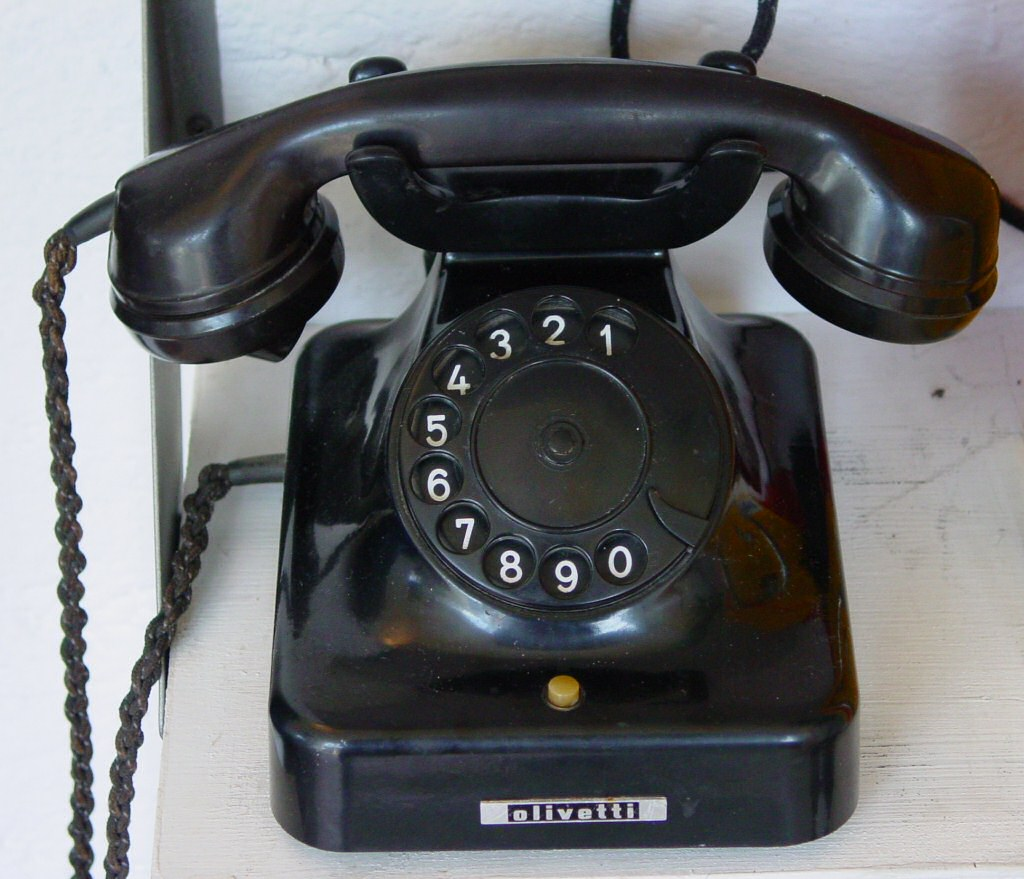
\includegraphics[width=\textwidth,height=1\textheight,keepaspectratio]{pics/phone.jpg}
\end{center}
\end{frame}

\section{Supported Systems}

\begin{frame}{Supported Systems}
\begin{itemize}
\item GitHub
\item Request Tracker
\item IMAP
\item Teamwork
\item Google Calendar
\end{itemize}
\end{frame}

\section{Configuration and Commandline}
\begin{frame}[fragile]{Configuration}
\begin{lstlisting}
inbox:
  type: imap
  server: ``support.linuxia.de''
  user: racke
  password: nevairbe
  ssl: 1
\end{lstlisting}
\end{frame}

\section{Forecast and Contribution}

\subsection{Slides}

\begin{frame}{Slides}
Slides:
\url{http://www.linuxia.de/talks/perldancer2014/helpdesk-en-beamer.pdf}
\end{frame}

\end{document}

%%% Local Variables: 
%%% mode: latex
%%% TeX-master: t
%%% End: 
